\documentclass[hyperref={pdfpagelabels=false}]{beamer}
% beamer already loads hyperref; do NOT load \usepackage{hyperref} again.

\usepackage{ragged2e} % 文字向兩邊對齊
\renewcommand{\raggedright}{\leftskip=0pt \rightskip=0pt plus 0cm}

\usepackage{listings}
\usepackage{lmodern}
\usepackage{fontspec}
\usepackage{xeCJK}
\setCJKmainfont{Noto Sans CJK TC}
\setCJKsansfont{Noto Sans CJK TC}
\setCJKmonofont{Noto Sans Mono CJK TC}

\usepackage[english]{babel}
\usepackage{amsmath,amssymb,amsfonts,amsthm}

\hypersetup{
  colorlinks=true,
  urlcolor=blue,
  citecolor=blue,
  pdfborder={0 0 0}
}

\usepackage{accsupp}
\newcommand{\emptyaccsupp}[1]{\BeginAccSupp{ActualText={}}#1\EndAccSupp{}}

\usepackage{tikz}
\usetikzlibrary{arrows,decorations.pathmorphing,backgrounds,fit,positioning,shapes.symbols,chains,trees,shapes.geometric}

\usepackage{booktabs}
\usepackage{threeparttable}
\usepackage{colortbl}
\usepackage{xcolor}
\usetikzlibrary{tikzmark}

\newcommand{\indep}{\perp\!\!\!\perp}
\newcommand{\nindep}{\not\!\perp\!\!\!\perp}

\beamertemplatefootpagenumber


\usepackage{listings}
%%%%%%%%%%%%%%%%%%%%%%%%%%%%%%%%%%%%%%%%%%%%%%%%%%%%%%%%%%%%%%%%%%%%%%%%%%%%%%
% Stata listings style
%%%%%%%%%%%%%%%%%%%%%%%%%%%%%%%%%%%%%%%%%%%%%%%%%%%%%%%%%%%%%%%%%%%%%%%%%%%%%%

\lstdefinelanguage{Stata}{
	morekeywords=,
	morekeywords=[2]{cntrade, chinafin, wbopendata, spmap,},
	morekeywords=[3]{regress, summarize, display,},
	morekeywords=[4]{forvalues, if, foreach, set},
	morekeywords=[5]{rnormal, runiform},
	morecomment=[l]{//},
	morecomment=[s]{/*}{*/},
	morecomment=[n][keywordstyle9]{`}{'},
	morestring=[b]",
	sensitive=true,
}

\lstdefinestyle{numbers}{
	numbers=left,
	stepnumber=1,
	numberstyle=\tiny\emptyaccsupp,
	xleftmargin=2em,
}

\lstdefinestyle{nonumbers}{
	numbers=none,
}

\lstdefinestyle{stata-plain}{
	language=Stata,
	basicstyle=\footnotesize\ttfamily,
}

\lstdefinestyle{stata-editor}{
	language=Stata,
	basicstyle=\footnotesize\ttfamily,
	keywordstyle={\color{NavyBlue}},
	keywordstyle=[2]{\color{NavyBlue}},
	keywordstyle=[3]{\color{NavyBlue}},
	keywordstyle=[4]{\color{NavyBlue}},
	keywordstyle=[5]{\color{Blue}},
	keywordstyle=[9]{\color{TealBlue}},
	stringstyle=\color{Maroon},
	commentstyle=\color{OliveGreen},
}

\lstset{
	language=Stata,
	style=stata-plain,
	style=numbers,
	showstringspaces=false,
	breaklines,
	frame=single,
}




\title[]
{Causal Machine Learning (III): Causal Forest}

\author
{Prof. Tzu-Ting Yang  \\ 楊子霆}

\institute{Institute of Economics, Academia Sinica  \\ 中央研究院經濟研究所}

\date
{\today}


\usetheme{CambridgeUS}
\setbeamertemplate{footline}{%
	\hfill\usebeamercolor[fg]{page number in head/foot}%
	\usebeamerfont{page number in head/foot}%
	\insertframenumber\,/\,\inserttotalframenumber\hspace{1em}\vspace{2pt}%
}

\beamersetuncovermixins{\opaqueness<1>{25}}{\opaqueness<2->{15}}

\begin{document}


\begin{frame}{}
	\titlepage
\end{frame}




%=============================================================
\title[]
{Main Idea}

\author{}
\institute{}
\date{}

\begin{frame}{}
	\titlepage
\end{frame}




% \begin{frame}{Causal Machine Learning: Series Overview}
% 	\begin{itemize}
% 		\item \textbf{Machine learning (ML)} methods use data-driven algorithms to model the relationship between an outcome \textbf{Y} and covariates \textbf{X}
% 		\vspace{0.2cm}
% 		\begin{itemize}
% 			\item There are many ML methods; \textbf{regression} is a fundamental one
% 			\vspace{0.2cm}
% 			\item The best method depends on the application
% 		\end{itemize}
% 		\vspace{0.3cm}
% 		\item For \textbf{causal inference}, ML methods help us identify treatment effects credibly
% 		\vspace{0.3cm}
% 		\item This lecture series covers three approaches:
% 		\vspace{0.2cm}
% 		\begin{itemize}
% 			\item \textbf{Part I:} Regression --- foundational ML tool for causal inference
% 			\vspace{0.2cm}
% 			\item \textbf{Part II:} Post-Double Selection --- high-dimensional covariates with LASSO
% 			\vspace{0.2cm}
% 			\item \textbf{Part III (This Lecture):} Heterogeneous Treatment Effects --- estimating CATE with Causal Forest
% 		\end{itemize}
% 	\end{itemize}
% \end{frame}




\begin{frame}{From Average to Heterogeneous Treatment Effects}
	\begin{itemize}
		\item Parts I and II focus on estimating the \textbf{Average Treatment Effect (ATE)}:
		\begin{equation*}
			\text{ATE} = \mathrm{E}[\mathrm{Y}^{1}_{i} - \mathrm{Y}^{0}_{i}]
		\end{equation*}

		\vspace{0.2cm}
		\item But the same policy may have \textbf{very different effects} for different people
		\vspace{0.2cm}
		\begin{itemize}
			\item A job training program may benefit low-educated workers more than college graduates
			\vspace{0.2cm}
			\item A minimum wage increase may hurt employment in some sectors but not others
			\vspace{0.2cm}
			\item Knowing \textbf{who benefits most} is crucial for targeting policies efficiently
		\end{itemize}
		\vspace{0.3cm}
		\item \textbf{Part III:} Estimate the \textbf{Conditional Average Treatment Effect (CATE)}:
		\begin{equation*}
			\tau(x) = \mathrm{E}[\mathrm{Y}^{1}_{i} - \mathrm{Y}^{0}_{i} \mid X_{i} = x]
		\end{equation*}
	\end{itemize}
\end{frame}




%=============================================================
\title[]
{From ATE to CATE}

\author{}
\institute{}
\date{}

\begin{frame}{}
	\titlepage
\end{frame}




\begin{frame}{Conditional Average Treatment Effect (CATE)}
	\begin{itemize}
		\item The \textbf{CATE} captures how treatment effects vary across individuals with different observed characteristics $X_i$
		\begin{equation*}
			\tau(x) = \mathrm{E}[\mathrm{Y}^{1}_{i} - \mathrm{Y}^{0}_{i} \mid X_{i} = x]
		\end{equation*}
		\vspace{0.2cm}
		\item $\tau(x)$ is a \textbf{function} of covariates $x$, not a single number
		\vspace{0.2cm}
		\begin{itemize}
			\item For example, $\tau(\text{age}=25, \text{educ}=12)$ may differ from $\tau(\text{age}=40, \text{educ}=16)$
		\end{itemize}
		\vspace{0.3cm}
		\item \textbf{Special cases:}
		\vspace{0.2cm}
		\begin{itemize}
			\item ATE $= \mathrm{E}[\tau(X_i)]$: average of CATE over the population
			\vspace{0.2cm}
			\item ATT $= \mathrm{E}[\tau(X_i) \mid D_i = 1]$: average CATE among the treated
		\end{itemize}
	\end{itemize}
\end{frame}




\begin{frame}{Why Can't Standard Regression Estimate CATE?}
	\begin{itemize}
		\item Standard regression assumes a \textbf{constant treatment effect}:
		\begin{equation*}
			\mathrm{Y}_i = \delta + \alpha D_i + X_i \beta + \epsilon_i
		\end{equation*}
		Here $\alpha$ is assumed the same for everyone
		\vspace{0.3cm}
		\item We can add \textbf{interaction terms} to allow heterogeneity:
		\begin{equation*}
			\mathrm{Y}_i = \delta + \alpha D_i + X_i \beta + (D_i \times X_i)\gamma + \epsilon_i
		\end{equation*}
		\vspace{0.2cm}
		\begin{itemize}
			\item But with many covariates $X$, this creates \textbf{too many interactions}
			\vspace{0.2cm}
			\item We do not know which interactions matter a priori
			\vspace{0.2cm}
			\item Standard regression cannot flexibly capture complex, nonlinear heterogeneity
		\end{itemize}
		\vspace{0.3cm}
		\item \textbf{Tree-based ML methods} can flexibly model $\tau(x)$ without specifying its functional form
	\end{itemize}
\end{frame}




\begin{frame}{Identifying CATE: Conditional Independence Assumption}
	\begin{block}{Conditional Independence Assumption (CIA)}
		\begin{equation*}
			(\mathrm{Y}^{1}_{i}, \mathrm{Y}^{0}_{i}) \indep D_{i} \mid X_{i}
		\end{equation*}
	\end{block}
	\begin{itemize}
		\vspace{0.3cm}
		\item Same assumption as in Parts I and II: treatment is \textbf{as good as random} after conditioning on observed covariates $X_i$
		\vspace{0.3cm}
		\item Under CIA, the CATE is identified:
		\begin{equation*}
			\tau(x) = \mathrm{E}[\mathrm{Y}_i \mid X_i = x, D_i = 1] - \mathrm{E}[\mathrm{Y}_i \mid X_i = x, D_i = 0]
		\end{equation*}
		\vspace{0.2cm}
		\item The challenge is estimating this difference \textbf{flexibly} for all values of $x$
	\end{itemize}
\end{frame}




%=============================================================
\title[]
{Decision Trees}

\author{}
\institute{}
\date{}

\begin{frame}{}
	\titlepage
\end{frame}




\begin{frame}{Decision Trees: Main Idea}
	\begin{itemize}
		\item A \textbf{decision tree} partitions the covariate space into rectangular regions, and fits a simple model (e.g., a mean) within each region
		\vspace{0.3cm}
		\item \textbf{Algorithm (Recursive Binary Splitting):}
		\vspace{0.2cm}
		\begin{itemize}
			\item[1] Find the variable $X^j$ and split point $s$ that minimizes prediction error
			\vspace{0.2cm}
			\item[2] Divide the data into two regions: $\{X^j < s\}$ and $\{X^j \geq s\}$
			\vspace{0.2cm}
			\item[3] Repeat within each region until a stopping rule is met
		\end{itemize}
		\vspace{0.3cm}
		\item The final estimate in each \textbf{leaf} (terminal node) is the mean of $Y$ for observations that fall in that leaf
	\end{itemize}
\end{frame}




\begin{frame}{Decision Trees: Finding the Best Split}
\textbf{How to find $(X^j,\, s)$ that minimises prediction error:}
\vspace{0.2cm}
\begin{enumerate}
  \item For each variable $X^j$ and each candidate split point $s$ (every observed value):
  \vspace{0.2cm}

  \begin{itemize}
    \item Divide data into two regions:
 

      $R_1(j,s) = \{i : X^j_i < s\}$ and $R_2(j,s) = \{i : X^j_i \geq s\}$
         \vspace{0.2cm}
    \item Compute the \textbf{residual sum of squares (RSS)} after the split:
    \begin{align*}
      \text{RSS}(j,s) \;=\;
      \sum_{i\in R_1}\!\bigl(Y_i - \bar{Y}_{R_1}\bigr)^2
      \;+\;
      \sum_{i\in R_2}\!\bigl(Y_i - \bar{Y}_{R_2}\bigr)^2
    \end{align*}
    where $\bar{Y}_{R_1},\bar{Y}_{R_2}$ are the mean $Y$ in each region\
    \vspace{0.2cm}

  \end{itemize}
  \item Choose the $(j^*, s^*)$ that gives the \textbf{smallest} $\text{RSS}(j,s)$
  \vspace{0.2cm}
  \item Repeat recursively inside each region
\end{enumerate}

% \vspace{0.2cm}
% \textbf{Common stopping rules (hyperparameters):}
% \vspace{0.1cm}

% \begin{tabular}{ll}
% \texttt{min\_node\_size} & Stop if a region has $<k$ observations (e.g.\ $k=5$) \\[3pt]
% \texttt{max\_depth}      & Stop after $d$ levels of splits (e.g.\ $d=5$) \\[3pt]
% \texttt{min\_decrease}   & Stop if best split reduces RSS by $<\varepsilon$ \\
% \end{tabular}

% \vspace{0.15cm}
% \begin{itemize}
%   \item These rules \textbf{prevent overfitting}: a tree that keeps splitting until every leaf has 1 observation perfectly fits training data but predicts nothing
% \end{itemize}
\end{frame}





\begin{frame}{Decision Trees: Finding the Best Split}
% \textbf{How to find $(X^j,\, s)$ that minimises prediction error:}
% \vspace{0.15cm}
% \begin{enumerate}
%   \item For each variable $X^j$ and each candidate split point $s$ (every observed value):
%   \begin{itemize}
%     \item Divide data into two regions:
%       $R_1(j,s) = \{i : X^j_i < s\}$ and $R_2(j,s) = \{i : X^j_i \geq s\}$
%     \item Compute the \textbf{residual sum of squares (RSS)} after the split:
%     \begin{align*}
%       \text{RSS}(j,s) \;=\;
%       \sum_{i\in R_1}\!\bigl(Y_i - \bar{Y}_{R_1}\bigr)^2
%       \;+\;
%       \sum_{i\in R_2}\!\bigl(Y_i - \bar{Y}_{R_2}\bigr)^2
%     \end{align*}
%     where $\bar{Y}_{R_1},\bar{Y}_{R_2}$ are the mean $Y$ in each region
%   \end{itemize}
%   \item Choose the $(j^*, s^*)$ that gives the \textbf{smallest} $\text{RSS}(j,s)$
%   \item Repeat recursively inside each region
% \end{enumerate}

% \vspace{0.2cm}
\textbf{Common stopping rules (hyperparameters):}
\vspace{0.1cm}

\begin{tabular}{ll}
\texttt{min\_node\_size} & Stop if a region has $<k$ observations (e.g.\ $k=5$) \\[3pt]
\texttt{max\_depth}      & Stop after $d$ levels of splits (e.g.\ $d=5$) \\[3pt]
\texttt{min\_decrease}   & Stop if best split reduces RSS by $<\varepsilon$ \\
\end{tabular}

\vspace{0.15cm}
\begin{itemize}
  \item These rules \textbf{prevent overfitting}: a tree that keeps splitting until every leaf has 1 observation perfectly fits training data but predicts nothing
\end{itemize}
\end{frame}





\begin{frame}{Decision Trees: Illustration}
	\begin{itemize}
		\item Suppose we want to predict wages $Y$ using age and education $X$
		\vspace{0.2cm}
		\begin{itemize}
			\item Split 1: age $< 30$ vs. age $\geq 30$
			\vspace{0.2cm}
			\item Split 2 (within age $\geq 30$): educ $< 12$ vs. educ $\geq 12$
		\end{itemize}
		\vspace{0.3cm}
		\item Each leaf contains observations with similar $X$ and similar predicted $Y$
		\vspace{0.3cm}
		\item \textbf{Advantages:}
		\vspace{0.2cm}
		\begin{itemize}
			\item Flexible: can capture nonlinear and interaction effects automatically
			\vspace{0.2cm}
			\item Interpretable: easy to visualize and explain
		\end{itemize}
		\vspace{0.3cm}
		\item \textbf{Disadvantage:} A single tree tends to \textbf{overfit} (high variance)
		\vspace{0.2cm}
		\begin{itemize}
			\item Solution: aggregate many trees (\textbf{Random Forest})
		\end{itemize}
	\end{itemize}
\end{frame}




\begin{frame}{Decision Trees: Tree Structure Example}
\begin{columns}[T]
	\begin{column}{0.52\textwidth}
		\begin{center}
		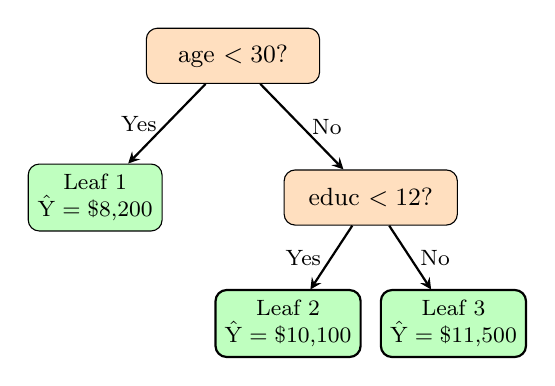
\begin{tikzpicture}[
			level 1/.style={sibling distance=3.5cm, level distance=1.8cm},
			level 2/.style={sibling distance=2.1cm, level distance=1.6cm},
			internal/.style={draw, rounded corners, fill=orange!25,
				align=center, font=\small,
				minimum width=2.2cm, minimum height=0.7cm},
			leaf/.style={draw, rounded corners, fill=green!25,
				align=center, font=\footnotesize,
				minimum width=1.7cm, minimum height=0.85cm},
			edge from parent/.style={draw, -stealth, thick}
		]
		\node[internal] {age $< 30$?}
			child {node[leaf] {Leaf 1\\ $\hat{\mathrm{Y}}=\$8{,}200$}
				edge from parent node[left, draw=none, fill=none,
					font=\footnotesize] {Yes}
			}
			child {node[internal] {educ $< 12$?}
				child {node[leaf] {Leaf 2\\ $\hat{\mathrm{Y}}=\$10{,}100$}
					edge from parent node[left, draw=none, fill=none,
						font=\footnotesize] {Yes}
				}
				child {node[leaf] {Leaf 3\\ $\hat{\mathrm{Y}}=\$11{,}500$}
					edge from parent node[right, draw=none, fill=none,
						font=\footnotesize] {No}
				}
				edge from parent node[right, draw=none, fill=none,
					font=\footnotesize] {No}
			};
		\end{tikzpicture}
		\end{center}
	\end{column}
	\begin{column}{0.48\textwidth}
		\small
		\begin{itemize}
			\item \textbf{Internal nodes} (orange): decision rules on $X$
			\vspace{0.2cm}
			\item \textbf{Leaves} (green): prediction $\hat{\mathrm{Y}}$ = mean of $\mathrm{Y}_i$ in that region
			\vspace{0.3cm}
			\item \textbf{Prediction}: follow branches until reaching a leaf
			\vspace{0.3cm}
			\item \textit{Example}: age $= 35$, educ $= 14$\\[4pt]
			$\rightarrow$ age $\geq 30$, educ $\geq 12$\\[2pt]
			$\rightarrow$ \textbf{Leaf 3}: $\hat{\mathrm{Y}} = \$11{,}500$
		\end{itemize}
	\end{column}
\end{columns}
\end{frame}




\begin{frame}{Decision Trees: Partition of Feature Space}
\begin{columns}[T]
	\begin{column}{0.52\textwidth}
		\vspace{0.3cm}
		\begin{center}
		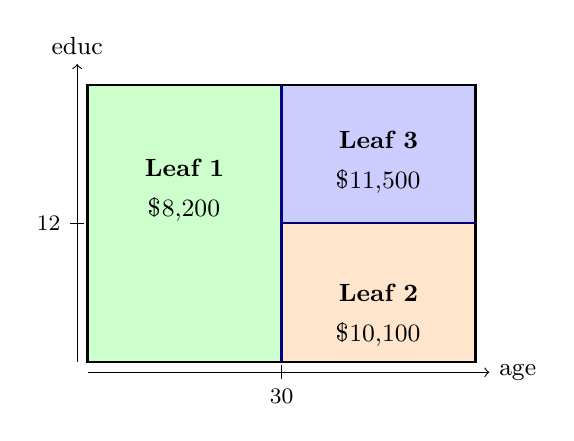
\begin{tikzpicture}[scale=0.88]
			% Fill regions first
			\fill[green!20]  (0,0) rectangle (2.8,4.0);
			\fill[orange!20] (2.8,0) rectangle (5.6,2.0);
			\fill[blue!20]   (2.8,2.0) rectangle (5.6,4.0);
			% Outer border
			\draw[thick] (0,0) rectangle (5.6,4.0);
			% Split 1: vertical at age=30
			\draw[thick, NavyBlue] (2.8,0) -- (2.8,4.0);
			% Split 2: horizontal at educ=12 (right half only)
			\draw[thick, NavyBlue] (2.8,2.0) -- (5.6,2.0);
			% Region labels
			\node[font={\small\bfseries}] at (1.4, 2.8) {Leaf 1};
			\node[font=\small] at (1.4, 2.2) {\$8,200};
			\node[font={\small\bfseries}] at (4.2, 1.0) {Leaf 2};
			\node[font=\small] at (4.2, 0.4) {\$10,100};
			\node[font={\small\bfseries}] at (4.2, 3.2) {Leaf 3};
			\node[font=\small] at (4.2, 2.6) {\$11,500};
			% Axes
			\draw[->] (0,-0.15) -- (5.8,-0.15) node[right, font=\small] {age};
			\draw[->] (-0.15,0) -- (-0.15,4.3) node[above, font=\small] {educ};
			% Axis ticks
			\draw (2.8,-0.05) -- (2.8,-0.25) node[below, font=\footnotesize] {30};
			\draw (-0.05,2.0) -- (-0.25,2.0) node[left, font=\footnotesize] {12};
		\end{tikzpicture}
		\end{center}
	\end{column}
	\begin{column}{0.48\textwidth}
		\small
		\begin{itemize}
			\item Each split divides the feature space into \textbf{rectangular regions}
			\vspace{0.3cm}
			\item All observations in the same region receive the \textbf{same prediction} (the in-region mean of $\mathrm{Y}$)
			\vspace{0.3cm}
			\item A \textbf{deeper tree} $\Rightarrow$ more splits $\Rightarrow$ smaller regions $\Rightarrow$ more flexible, but risks \textbf{overfitting}
			\vspace{0.3cm}
			\item The tree approximates any nonlinear relationship between $\mathrm{Y}$ and $X$ without specifying a functional form
		\end{itemize}
	\end{column}
\end{columns}
\end{frame}




%=============================================================
\title[]
{Random Forest}

\author{}
\institute{}
\date{}

\begin{frame}{}
	\titlepage
\end{frame}




\begin{frame}{Why a Single Decision Tree Is Not Enough}
	\begin{itemize}
		\item A single deep tree has a fundamental weakness: \textbf{high variance}
		\vspace{0.3cm}
		\begin{itemize}
			\item The tree ``memorizes'' the training data rather than learning the true pattern
			\vspace{0.2cm}
			\item Small changes in the data (e.g.\ adding or removing a few observations) can lead to a completely different tree structure
			\vspace{0.2cm}
			\item Predictions on new data are unstable and often poor
		\end{itemize}
		\vspace{0.3cm}
		\item \textbf{Intuition:} Like asking one person for an opinion --- noisy and unreliable
		\vspace{0.3cm}
		\item \textbf{Solution:} Ask many people independently and take the average
		\vspace{0.2cm}
		\begin{itemize}
			\item In ML: grow many diverse trees on different random subsamples and average their predictions
			\item This is \textbf{Random Forest} (Breiman, 2001)
		\end{itemize}
	\end{itemize}
\end{frame}




\begin{frame}{High Variance: One Small Change, Completely Different Tree}
\begin{center}
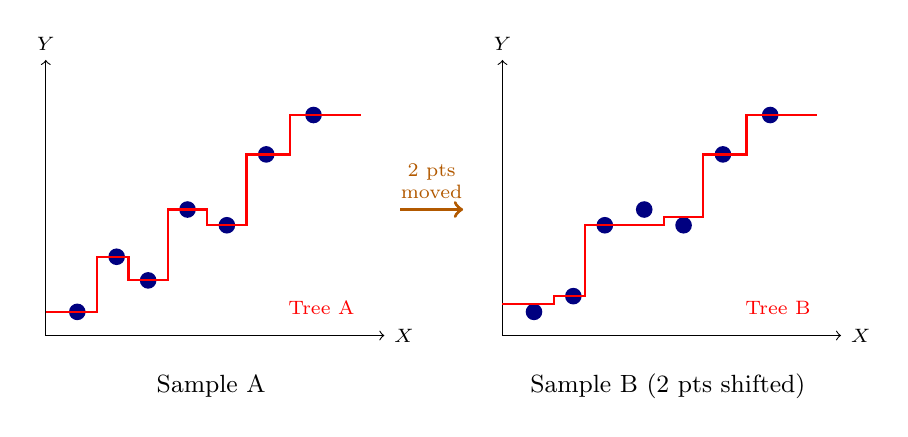
\begin{tikzpicture}
	% ---- Left panel: Sample A ----
	\begin{scope}
		\draw[->] (0,0) -- (4.3,0) node[right, font=\scriptsize] {$X$};
		\draw[->] (0,0) -- (0,3.5) node[above, font=\scriptsize] {$Y$};
		\node[font=\small, align=center] at (2.1,-0.65) {Sample A};
		% Data points
		\foreach \x/\y in {0.4/0.3, 0.9/1.0, 1.3/0.7, 1.8/1.6, 2.3/1.4, 2.8/2.3, 3.4/2.8}
			\fill[NavyBlue] (\x,\y) circle (3pt);
		% Deep tree (step function, memorising every point)
		\draw[red,thick]
			(0,0.3)--(0.65,0.3)--(0.65,1.0)--(1.05,1.0)--(1.05,0.7)
			--(1.55,0.7)--(1.55,1.6)--(2.05,1.6)--(2.05,1.4)
			--(2.55,1.4)--(2.55,2.3)--(3.1,2.3)--(3.1,2.8)--(4.0,2.8);
		\node[red,font=\scriptsize] at (3.5,0.35) {Tree A};
	\end{scope}

	% ---- Arrow ----
	\draw[->,very thick,orange!70!black] (4.5,1.6)--(5.3,1.6)
		node[midway,above,font=\scriptsize,align=center,orange!70!black]
		{2 pts\\moved};

	% ---- Right panel: Sample B ----
	\begin{scope}[xshift=5.8cm]
		\draw[->] (0,0) -- (4.3,0) node[right, font=\scriptsize] {$X$};
		\draw[->] (0,0) -- (0,3.5) node[above, font=\scriptsize] {$Y$};
		\node[font=\small, align=center] at (2.1,-0.65) {Sample B (2 pts shifted)};
		% Slightly different data (2 observations moved)
		\foreach \x/\y in {0.4/0.3, 0.9/0.5, 1.3/1.4, 1.8/1.6, 2.3/1.4, 2.8/2.3, 3.4/2.8}
			\fill[NavyBlue] (\x,\y) circle (3pt);
		% Completely different tree
		\draw[red,thick]
			(0,0.4)--(0.65,0.4)--(0.65,0.5)--(1.05,0.5)
			--(1.05,1.4)--(2.05,1.4)--(2.05,1.5)
			--(2.55,1.5)--(2.55,2.3)--(3.1,2.3)--(3.1,2.8)--(4.0,2.8);
		\node[red,font=\scriptsize] at (3.5,0.35) {Tree B};
	\end{scope}
\end{tikzpicture}
\end{center}
\vspace{0.1cm}
\begin{itemize}
	\item A tiny change in the data $\Rightarrow$ \textbf{completely different splits} $\Rightarrow$ highly unstable predictions
	\item[$\Rightarrow$] We need to average over many trees to stabilise: \textbf{Random Forest}
\end{itemize}
\end{frame}




\begin{frame}{Random Forest: How It Works}
\begin{columns}[T]
	\begin{column}{0.50\textwidth}
		\small
		\textbf{Algorithm:} Repeat $B$ times---
		\vspace{0.2cm}
		\begin{itemize}
			\item[1.] Draw a \textbf{random subsample} from the data (typically without replacement)
			\vspace{0.2cm}
			\item[2.] Grow a deep decision tree, but at each split only consider a \textbf{random subset of $m$ covariates} (e.g.\ $m=\sqrt{p}$)
		\end{itemize}
		\vspace{0.3cm}
		\textbf{Prediction for a new $x$:}
		\begin{equation*}
			\hat{\mathrm{Y}}(x) = \frac{1}{B}\sum_{b=1}^{B} \hat{\mathrm{Y}}_{b}(x)
		\end{equation*}
		average over all $B$ trees
	\end{column}
	\begin{column}{0.50\textwidth}
		\small
		\textbf{Why does this reduce variance?}
		\vspace{0.2cm}
		\begin{itemize}
			\item If $B$ independent trees each have variance $\sigma^2$, their average has variance $\sigma^2/B$
			\vspace{0.2cm}
			\item Trees are not fully independent, but random subsampling $+$ feature randomness makes them \textbf{diverse} $\Rightarrow$ low correlation $\Rightarrow$ big variance reduction
		\end{itemize}
		\vspace{0.3cm}
		\begin{tabular}{lcc}
			\toprule
			 & Bias & Variance \\
			\midrule
			Single tree & Low & \textbf{High} \\
			Random Forest & Low & \textbf{Low} \\
			\bottomrule
		\end{tabular}
	\end{column}
\end{columns}
\end{frame}




\begin{frame}{Random Forest: Illustration}
\begin{center}
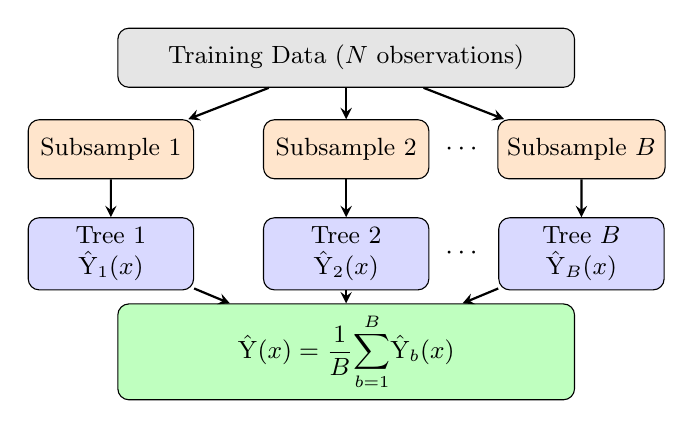
\begin{tikzpicture}[scale=0.83,
	box/.style={draw, rounded corners, minimum width=2.1cm, minimum height=0.75cm,
		align=center, font=\small},
	arr/.style={-stealth, thick}
]
	% Full dataset
	\node[box, fill=gray!20, minimum width=5.8cm] (data) at (0, 4.2)
		{Training Data ($N$ observations)};

	% Subsamples
	\node[box, fill=orange!20] (s1) at (-3.6, 2.8) {Subsample 1};
	\node[box, fill=orange!20] (s2) at (0,    2.8) {Subsample 2};
	\node[box, fill=orange!20] (s3) at (3.6,  2.8) {Subsample $B$};
	\node at (1.8, 2.8) {$\cdots$};

	\draw[arr] (data) -- (s1);
	\draw[arr] (data) -- (s2);
	\draw[arr] (data) -- (s3);

	% Trees
	\node[box, fill=blue!15] (t1) at (-3.6, 1.2)
		{Tree 1\\ $\hat{\mathrm{Y}}_1(x)$};
	\node[box, fill=blue!15] (t2) at (0,    1.2)
		{Tree 2\\ $\hat{\mathrm{Y}}_2(x)$};
	\node[box, fill=blue!15] (t3) at (3.6,  1.2)
		{Tree $B$\\ $\hat{\mathrm{Y}}_B(x)$};
	\node at (1.8, 1.2) {$\cdots$};

	\draw[arr] (s1) -- (t1);
	\draw[arr] (s2) -- (t2);
	\draw[arr] (s3) -- (t3);

	% Average prediction
	\node[box, fill=green!25, minimum width=5.8cm] (avg) at (0, -0.3)
		{$\hat{\mathrm{Y}}(x)=\dfrac{1}{B}{\displaystyle\sum_{b=1}^{B}}\hat{\mathrm{Y}}_{b}(x)$};

	\draw[arr] (t1) -- (avg);
	\draw[arr] (t2) -- (avg);
	\draw[arr] (t3) -- (avg);
\end{tikzpicture}
\end{center}
\vspace{-0.2cm}
\begin{itemize}
	\item Each tree is grown on a different subsample $\Rightarrow$ trees are diverse and their errors tend to cancel
\end{itemize}
\end{frame}




\begin{frame}{From Prediction to Causal Inference}
	\begin{itemize}
		\item Random Forest is a powerful tool for \textbf{prediction}: estimating $\mathrm{E}[\mathrm{Y}_i \mid X_i = x]$
		\vspace{0.3cm}
		\item But we often want more: \textbf{what is the causal effect of treatment $D_i$ on $\mathrm{Y}_i$ for different types of people?}
		\vspace{0.3cm}
		\item To answer this, we need trees designed to estimate the \textbf{treatment effect}, not just the outcome
		\vspace{0.3cm}
		\item \textbf{Problem:} Applying a standard decision tree to causal inference introduces a new bias --- even beyond overfitting
		\vspace{0.2cm}
		\begin{itemize}
			\item The tree searches for splits where the treatment effect \textit{looks} large
			\vspace{0.2cm}
			\item Estimating effects in the same data that was used to find the splits inflates estimates
		\end{itemize}
		\vspace{0.3cm}
		\item[$\Rightarrow$] We need a \textbf{Causal Tree} (Athey \& Imbens, 2016)
	\end{itemize}
\end{frame}




\begin{frame}{Naive Tree for Causal Inference: The Goal}
	\begin{itemize}
		\item When building a \textbf{causal tree}, we want to find subgroups where the treatment effect $\tau(x)$ is large versus small
		\vspace{0.3cm}
		\item \textbf{Natural algorithm:}
		\vspace{0.2cm}
		\begin{itemize}
			\item[1.] Try every possible split on every covariate $X^j$
			\vspace{0.2cm}
			\item[2.] Pick the split that makes the treatment effect \textbf{most different} across the two resulting leaves
			\vspace{0.2cm}
			\item[3.] Estimate $\hat{\tau}(\ell)$ in each leaf: mean of treated $-$ mean of control
			\vspace{0.2cm}
			\item[4.] Repeat recursively until leaves are small enough
		\end{itemize}
		\vspace{0.3cm}
		\item \textbf{Problem:} Steps 2 and 3 use the \textbf{same data} --- this introduces bias
	\end{itemize}
\end{frame}


\begin{frame}{Naive Tree: Why the Estimates are Biased}
\begin{columns}[T]
	\begin{column}{0.50\textwidth}
		\small
		\textbf{Scenario:} 8 workers, training vs.\ no training.
		We try splitting on \textit{age $<$ 30}.

		\vspace{0.4cm}
		\begin{tabular}{lcc}
			\toprule
			 & Treated & Control \\
			\midrule
			age $< 30$ & \$9,500 & \$7,000 \\
			age $\geq 30$ & \$9,200 & \$8,800 \\
			\bottomrule
		\end{tabular}

		\vspace{0.4cm}
		\footnotesize
		Estimated effect:\\[3pt]
		\quad age $< 30$: $\$9{,}500 - \$7{,}000 = \mathbf{\$2{,}500}$\\[3pt]
		\quad age $\geq 30$: $\$9{,}200 - \$8{,}800 = \mathbf{\$400}$
	\end{column}
	\begin{column}{0.50\textwidth}
		\small
		\textbf{The bias:}
		\vspace{0.2cm}
		\begin{itemize}
			\item The tree selected \textit{age $= 30$} because the effect \textbf{looked large} in this leaf
			\vspace{0.2cm}
			\item But this large gap may be \textbf{noise} --- by searching many splits, we find ones that look big by chance
			\vspace{0.2cm}
			\item Then we \textbf{report \$2,500} for ``age $< 30$'' using the \textit{same} data that generated this lucky finding
			\vspace{0.2cm}
			\item True effect may be much smaller --- the estimate is \textbf{inflated upward}
		\end{itemize}
	\end{column}
\end{columns}
\end{frame}




\begin{frame}{Naive Tree: The Tree Searches for the ``Luckiest'' Split}
\begin{columns}[T]
	\begin{column}{0.54\textwidth}
		\begin{center}
		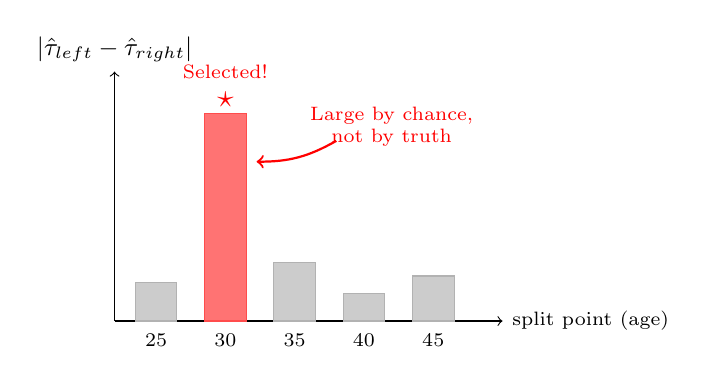
\begin{tikzpicture}[scale=0.88]
			% Y axis
			\draw[->] (0,0) -- (0,3.6)
				node[above, font=\small, align=center]
				{$|\hat{\tau}_{left} - \hat{\tau}_{right}|$};
			% X axis
			\draw[->] (0,0) -- (5.6,0)
				node[right, font=\scriptsize] {split point (age)};

			% Bar: age=25 (small)
			\fill[gray!40]  (0.3,0) rectangle (0.9, 0.55);
			\draw[gray!60]  (0.3,0) rectangle (0.9, 0.55);
			\node[font=\scriptsize,below] at (0.6,-0.05) {25};

			% Bar: age=30 --- SELECTED (large by chance)
			\fill[red!55]   (1.3,0) rectangle (1.9, 3.0);
			\draw[red!70]   (1.3,0) rectangle (1.9, 3.0);
			\node[font=\scriptsize,below] at (1.6,-0.05) {30};
			\node[red,font=\large]        at (1.6, 3.2) {$\star$};
			\node[red,font=\scriptsize, align=center] at (1.6, 3.6) {Selected!};

			% Bar: age=35 (small)
			\fill[gray!40]  (2.3,0) rectangle (2.9, 0.85);
			\draw[gray!60]  (2.3,0) rectangle (2.9, 0.85);
			\node[font=\scriptsize,below] at (2.6,-0.05) {35};

			% Bar: age=40 (very small)
			\fill[gray!40]  (3.3,0) rectangle (3.9, 0.4);
			\draw[gray!60]  (3.3,0) rectangle (3.9, 0.4);
			\node[font=\scriptsize,below] at (3.6,-0.05) {40};

			% Bar: age=45 (small)
			\fill[gray!40]  (4.3,0) rectangle (4.9, 0.65);
			\draw[gray!60]  (4.3,0) rectangle (4.9, 0.65);
			\node[font=\scriptsize,below] at (4.6,-0.05) {45};

			% Annotation arrow
			\draw[->,red,thick] (3.2,2.6) to[bend left=15] (2.05,2.3);
			\node[red,font=\scriptsize,align=center] at (4.0,2.8)
				{Large by chance,\\not by truth};
		\end{tikzpicture}
		\end{center}
	\end{column}
	\begin{column}{0.46\textwidth}
		\small
		\begin{itemize}
			\item The tree evaluates \textbf{every} candidate split on every covariate
			\vspace{0.2cm}
			\item Like testing 50 hypotheses: \textbf{at least one will look large by noise}
			\vspace{0.2cm}
			\item The tree selects age $=30$ because it appears largest \textbf{in this sample}
			\vspace{0.2cm}
			\item Then the \textbf{same data} reports $\hat{\tau}=\$2{,}500$ for the ``age$<30$'' leaf
			\vspace{0.2cm}
			\item $\Rightarrow$ estimate is \textbf{biased upward}: selected \textit{because} it looked large
		\end{itemize}
	\end{column}
\end{columns}
\end{frame}


\begin{frame}{Naive Tree: The ``Double-Dipping'' Problem}
	\begin{itemize}
		\item The problem is called \textbf{double-dipping}: using the same data twice
		\vspace{0.3cm}
		\begin{itemize}
			\item \textbf{First dip:} use the data to \textit{search} for splits where treatment effects look large
			\vspace{0.2cm}
			\item \textbf{Second dip:} use the \textit{same} data to \textit{measure} how large the effect is
		\end{itemize}
		\vspace{0.3cm}
		\item \textbf{Analogy:} A researcher tests 50 different subgroups and reports only the one with the largest effect --- but uses the same sample to estimate it
		\vspace{0.2cm}
		\begin{itemize}
			\item The reported effect is \textbf{cherry-picked} from noise
			\vspace{0.2cm}
			\item This is a form of \textbf{multiple testing bias} / data snooping
		\end{itemize}
		\vspace{0.3cm}
		\item \textbf{Solution:} Keep the \textit{search} and the \textit{measurement} on \textbf{separate samples}
		\vspace{0.2cm}
		\begin{itemize}
			\item This is the key idea of \textbf{Honest Estimation} (Athey \& Imbens, 2016)
		\end{itemize}
	\end{itemize}
\end{frame}




%=============================================================
\title[]
{Causal Tree}

\author{}
\institute{}
\date{}

\begin{frame}{}
	\titlepage
\end{frame}




\begin{frame}{Causal Tree}{Athey \& Imbens (2016)}
	Athey, Susan and Guido Imbens (2016), ``\textbf{Recursive Partitioning for Heterogeneous Causal Effects}'', \textit{Proceedings of the National Academy of Sciences}

	\vspace{0.3cm}
	\begin{itemize}
		\item Propose a \textbf{Causal Tree}: a decision tree designed to estimate \textbf{CATE}
		\vspace{0.2cm}
		\item Key innovation: \textbf{Honest Estimation}
		\vspace{0.2cm}
		\begin{itemize}
			\item Separate the data used for building the tree structure from the data used to estimate treatment effects within leaves
			\vspace{0.2cm}
			\item This eliminates the adaptive bias of naive trees
		\end{itemize}
		\vspace{0.3cm}
		\item Under CIA and honesty, within-leaf estimates of CATE are \textbf{unbiased}
	\end{itemize}
\end{frame}




\begin{frame}{Causal Tree: How Treatment Effects Are Estimated in Each Leaf}
\begin{columns}[T]
	\begin{column}{0.52\textwidth}
		\begin{center}
		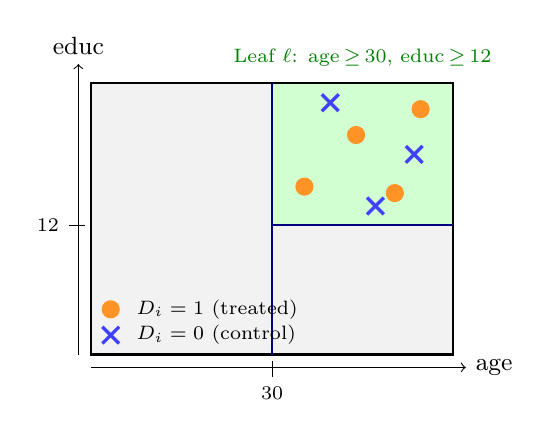
\begin{tikzpicture}[scale=0.82]
			% Background leaves (faded)
			\fill[gray!10] (0,0) rectangle (2.8,4.2);
			\fill[gray!10] (2.8,0) rectangle (5.6,2.0);
			% Highlighted leaf: age>=30, educ>=12
			\fill[green!18] (2.8,2.0) rectangle (5.6,4.2);
			\draw[thick, green!55!black] (2.8,2.0) rectangle (5.6,4.2);
			% Outer border + split lines
			\draw[thick] (0,0) rectangle (5.6,4.2);
			\draw[NavyBlue,thick] (2.8,0) -- (2.8,4.2);
			\draw[NavyBlue,thick] (2.8,2.0) -- (5.6,2.0);
			% Leaf label
			\node[font=\scriptsize, green!50!black, align=center]
				at (4.2,4.6) {Leaf $\ell$: age$\,\geq\,$30, educ$\,\geq\,$12};
			% Treated (orange filled circles)
			\foreach \x/\y in {3.3/2.6, 4.1/3.4, 4.7/2.5, 5.1/3.8}
				\fill[orange!85] (\x,\y) circle (4pt);
			% Control (blue crosses)
			\foreach \x/\y in {3.7/3.9, 4.4/2.3, 5.0/3.1} {
				\draw[blue!75,very thick] (\x-0.13,\y-0.13)--(\x+0.13,\y+0.13);
				\draw[blue!75,very thick] (\x+0.13,\y-0.13)--(\x-0.13,\y+0.13);
			}
			% Axes
			\draw[->] (0,-0.2)--(5.8,-0.2) node[right,font=\small] {age};
			\draw[->] (-0.2,0)--(-0.2,4.5) node[above,font=\small] {educ};
			\draw (2.8,-0.1)--(2.8,-0.35) node[below,font=\scriptsize] {30};
			\draw (-0.1,2.0)--(-0.35,2.0) node[left,font=\scriptsize] {12};
			% Legend
			\fill[orange!85] (0.3,0.7) circle (4pt);
			\node[font=\scriptsize,right] at (0.55,0.7) {$D_i=1$ (treated)};
			\draw[blue!75,very thick] (0.17,0.17)--(0.43,0.43);
			\draw[blue!75,very thick] (0.43,0.17)--(0.17,0.43);
			\node[font=\scriptsize,right] at (0.55,0.3) {$D_i=0$ (control)};
		\end{tikzpicture}
		\end{center}
	\end{column}
	\begin{column}{0.48\textwidth}
		\small
		Within leaf $\ell$ (age$\geq 30$, educ$\geq 12$):
		\vspace{0.25cm}
		\begin{itemize}
			\item 4 treated (\textcolor{orange!85!black}{$\bullet$}): $\;\bar{Y}^{1}_\ell = \$11{,}800$
			\vspace{0.1cm}
			\item 3 control ({\color{blue!75}$\times$}): $\quad\bar{Y}^{0}_\ell = \$10{,}200$
		\end{itemize}
		\begin{equation*}
			\hat{\tau}(\ell) = 11{,}800 - 10{,}200 = \mathbf{\$1{,}600}
		\end{equation*}
		\vspace{0.15cm}
		\begin{itemize}
			\item All units in the leaf have \textbf{similar} $X$ (same age \& educ range)
			\vspace{0.2cm}
			\item Under CIA, treated and control \textit{within} the leaf are comparable $\Rightarrow$ like a \textbf{local experiment}
			\vspace{0.2cm}
			\item The causal tree assigns $\hat{\tau}(x) = \hat{\tau}(\ell)$ to every individual $x$ that falls into leaf $\ell$
		\end{itemize}
	\end{column}
\end{columns}
\end{frame}




\begin{frame}{Honest Estimation: The Solution}
	\begin{itemize}
		\item \textbf{Key idea:} Randomly split the data into two halves and assign each half a separate role
		\vspace{0.3cm}
		\item \textbf{Step 1 --- Training sample $\mathcal{S}^{tr}$ (find splits only):}
		\vspace{0.2cm}
		\begin{itemize}
			\item Search for splits that create leaves with different treatment effects
			\vspace{0.2cm}
			\item Fix the \textbf{tree structure}: which variables to split on, and where
			\vspace{0.2cm}
			\item \textit{Do not compute treatment effects here}
		\end{itemize}
		\vspace{0.3cm}
		\item \textbf{Step 2 --- Estimation sample $\mathcal{S}^{est}$ (measure effects only):}
		\vspace{0.2cm}
		\begin{itemize}
			\item Drop each observation into the leaf it belongs to (using the tree from Step 1)
			\vspace{0.2cm}
			\item Estimate $\hat{\tau}(\ell)$ = mean outcome of treated $-$ mean outcome of control:
			\begin{equation*}
				\hat{\tau}(\ell) = \frac{1}{n^{1}_\ell} \sum_{\substack{i \in \mathcal{S}^{est}\\ i \in \ell,\, D_i=1}} \mathrm{Y}_i \;-\; \frac{1}{n^{0}_\ell} \sum_{\substack{i \in \mathcal{S}^{est}\\ i \in \ell,\, D_i=0}} \mathrm{Y}_i
			\end{equation*}
		\end{itemize}
		\vspace{0.2cm}
		\item \textbf{Why unbiased?} $\mathcal{S}^{est}$ had no role in choosing splits $\Rightarrow$ no cherry-picking
	\end{itemize}
\end{frame}




\begin{frame}{Honest Estimation: Illustration}
\begin{center}
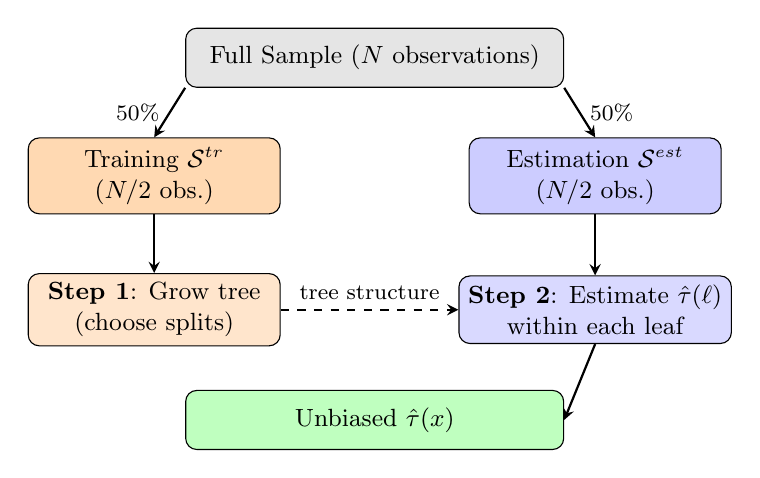
\begin{tikzpicture}[
	box/.style={draw, rounded corners, minimum width=3.2cm, minimum height=0.75cm,
		align=center, font=\small},
	arr/.style={-stealth, thick}
]
	% Full sample at top
	\node[box, fill=gray!20, minimum width=4.8cm] (data) at (0, 4)
		{Full Sample ($N$ observations)};

	% Two subsamples
	\node[box, fill=orange!30] (train) at (-2.8, 2.5)
		{Training $\mathcal{S}^{tr}$\\ ($N/2$ obs.)};
	\node[box, fill=blue!20]   (est)   at ( 2.8, 2.5)
		{Estimation $\mathcal{S}^{est}$\\ ($N/2$ obs.)};

	\draw[arr] (data.south west) -- (train.north)
		node[midway, left, font=\footnotesize] {50\%};
	\draw[arr] (data.south east) -- (est.north)
		node[midway, right, font=\footnotesize] {50\%};

	% Step 1: grow tree
	\node[box, fill=orange!20] (grow) at (-2.8, 0.8)
		{\textbf{Step 1}: Grow tree\\ (choose splits)};
	\draw[arr] (train) -- (grow);

	% Step 2: estimate within leaves
	\node[box, fill=blue!15]  (leaf) at (2.8, 0.8)
		{\textbf{Step 2}: Estimate $\hat{\tau}(\ell)$\\ within each leaf};
	\draw[arr] (est) -- (leaf);

	% Tree structure passes to estimation step
	\draw[arr, dashed] (grow.east) -- (leaf.west)
		node[midway, above, font=\footnotesize] {tree structure};

	% Output
	\node[box, fill=green!25, minimum width=4.8cm] (out) at (0, -0.6)
		{Unbiased $\hat{\tau}(x)$};
	\draw[arr] (leaf.south) -- (out.east);
\end{tikzpicture}
\end{center}
\vspace{-0.2cm}
\begin{itemize}
	\item Splitting the data eliminates \textbf{adaptive bias}: the tree cannot ``overfit'' to the same observations used to estimate effects
\end{itemize}
\end{frame}




\begin{frame}{Causal Tree: Summary}
	\begin{itemize}
		\item A causal tree assigns each individual a CATE estimate based on the leaf they fall into:
		\begin{equation*}
			\hat{\tau}(x) = \hat{\tau}(\ell(x))
		\end{equation*}
		where $\ell(x)$ is the leaf containing $x$
		\vspace{0.3cm}
		\item \textbf{Limitation of a single tree:}
		\vspace{0.2cm}
		\begin{itemize}
			\item High variance --- small changes in data can change the tree structure substantially
			\vspace{0.2cm}
			\item Each leaf contains few observations, leading to noisy estimates
		\end{itemize}
		\vspace{0.3cm}
		\item Solution: grow many causal trees and average their predictions --- \textbf{Causal Forest}
	\end{itemize}
\end{frame}




\begin{frame}{From Causal Tree to Causal Forest}
\begin{center}
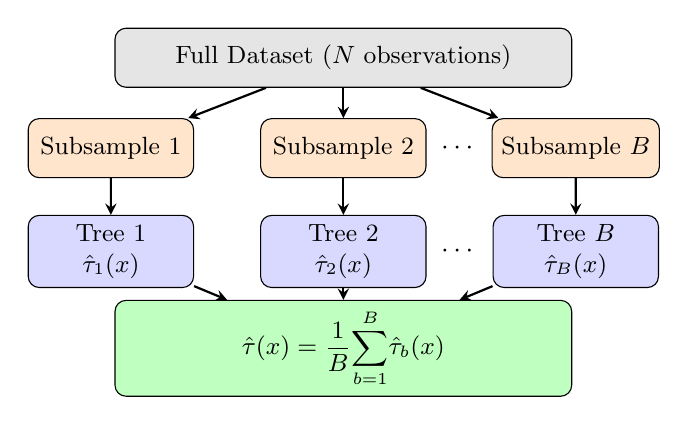
\begin{tikzpicture}[scale=0.82,
	box/.style={draw, rounded corners, minimum width=2.1cm, minimum height=0.75cm,
		align=center, font=\small},
	arr/.style={-stealth, thick}
]
	% Full dataset at top
	\node[box, fill=gray!20, minimum width=5.8cm] (data) at (0, 4.2)
		{Full Dataset ($N$ observations)};

	% Subsamples
	\node[box, fill=orange!20] (s1) at (-3.6, 2.8) {Subsample 1};
	\node[box, fill=orange!20] (s2) at (0,    2.8) {Subsample 2};
	\node[box, fill=orange!20] (s3) at (3.6,  2.8) {Subsample $B$};
	\node at (1.8, 2.8) {$\cdots$};

	\draw[arr] (data) -- (s1);
	\draw[arr] (data) -- (s2);
	\draw[arr] (data) -- (s3);

	% Trees
	\node[box, fill=blue!15] (t1) at (-3.6, 1.2)
		{Tree 1\\ $\hat{\tau}_1(x)$};
	\node[box, fill=blue!15] (t2) at (0,    1.2)
		{Tree 2\\ $\hat{\tau}_2(x)$};
	\node[box, fill=blue!15] (t3) at (3.6,  1.2)
		{Tree $B$\\ $\hat{\tau}_B(x)$};
	\node at (1.8, 1.2) {$\cdots$};

	\draw[arr] (s1) -- (t1);
	\draw[arr] (s2) -- (t2);
	\draw[arr] (s3) -- (t3);

	% Average
	\node[box, fill=green!25, minimum width=5.8cm] (avg) at (0, -0.3)
		{$\hat{\tau}(x)=\dfrac{1}{B}{\displaystyle\sum_{b=1}^{B}}\hat{\tau}_{b}(x)$};

	\draw[arr] (t1) -- (avg);
	\draw[arr] (t2) -- (avg);
	\draw[arr] (t3) -- (avg);
\end{tikzpicture}
\end{center}
\vspace{-0.2cm}
\begin{itemize}
	\item Same idea as Random Forest, but each tree estimates \textbf{treatment effects} $\hat{\tau}_b(x)$, not just outcomes $\hat{Y}_b(x)$
	\item Random subsamples $+$ feature randomness $\Rightarrow$ \textbf{diverse trees} $\Rightarrow$ averaging cancels noise $\Rightarrow$ lower variance
\end{itemize}
\end{frame}




%=============================================================
\title[]
{Causal Forest}

\author{}
\institute{}
\date{}

\begin{frame}{}
	\titlepage
\end{frame}




\begin{frame}{Causal Forest}{Wager \& Athey (2018)}
	Wager, Stefan and Susan Athey (2018), ``\textbf{Estimation and Inference of Heterogeneous Treatment Effects using Random Forests}'', \textit{Journal of the American Statistical Association}

	\vspace{0.3cm}
	\begin{itemize}
		\item Generalize Random Forest to estimate \textbf{CATE}
		\vspace{0.2cm}
		\begin{itemize}
			\item Build \textbf{many honest causal trees}, each using a random subsample and random subset of covariates
			\vspace{0.2cm}
			\item Average the CATE estimates across trees
		\end{itemize}
		\vspace{0.3cm}
		\item \textbf{Key theoretical results:}
		\vspace{0.2cm}
		\begin{itemize}
			\item \textbf{Consistency:} $\hat{\tau}(x) \xrightarrow{p} \tau(x)$ as sample size grows
			\vspace{0.2cm}
			\item \textbf{Asymptotic normality:} allows construction of valid confidence intervals for $\tau(x)$
		\end{itemize}
	\end{itemize}
\end{frame}




\begin{frame}{Causal Forest: Intuition}
	\begin{itemize}
		\item The causal forest implicitly assigns \textbf{weights} $\alpha_i(x)$ to each observation $i$ when predicting $\tau(x)$
		\vspace{0.2cm}
		\begin{itemize}
			\item $\alpha_i(x)$ is large if observation $i$ tends to fall in the same leaf as $x$ across many trees
			\vspace{0.2cm}
			\item Observations with $X_i$ similar to $x$ receive higher weight
		\end{itemize}
		\vspace{0.3cm}
		\item The CATE estimate at $x$ is essentially a \textbf{locally weighted comparison} of treated and control observations:
		\begin{equation*}
			\hat{\tau}(x) \approx \frac{\sum_i \alpha_i(x) \cdot (\mathrm{Y}_i - \bar{\mathrm{Y}}) \cdot (D_i - \bar{D})}{\sum_i \alpha_i(x) \cdot (D_i - \bar{D})^2}
		\end{equation*}
		\item This is like running a \textbf{local linear regression} of $Y$ on $D$, using the forest to define ``local neighborhood'' around $x$
	\end{itemize}
\end{frame}




\begin{frame}{Causal Forest: Key Assumption}
	\begin{itemize}
		\item Causal Forest still requires \textbf{CIA (selection on observables)}:
		\begin{equation*}
			(\mathrm{Y}^{1}_{i}, \mathrm{Y}^{0}_{i}) \indep D_{i} \mid X_{i}
		\end{equation*}
		\vspace{0.2cm}
		\item Additionally requires \textbf{overlap}: both treated and control units exist for all values of $X$
		\begin{equation*}
			0 < P(D_i = 1 \mid X_i = x) < 1 \quad \forall x
		\end{equation*}
		\vspace{0.3cm}
		\item \textbf{Comparison to Parts I and II:}
		\vspace{0.2cm}
		\begin{itemize}
			\item Same identification assumption (CIA)
			\vspace{0.2cm}
			\item Part I (Regression): assumes \textbf{linear, constant} treatment effect
			\vspace{0.2cm}
			\item Part II (PDS): focuses on ATE with high-dimensional controls
			\vspace{0.2cm}
			\item \textbf{Part III (Causal Forest): flexible nonlinear CATE estimation}
		\end{itemize}
	\end{itemize}
\end{frame}




\begin{frame}{Causal Forest: Literature}
	\begin{itemize}
		\item[] Athey, Susan and Guido Imbens (2016), ``\textbf{Recursive Partitioning for Heterogeneous Causal Effects}'', \textit{PNAS}
		\vspace{0.2cm}
		\item[] Wager, Stefan and Susan Athey (2018), ``\textbf{Estimation and Inference of Heterogeneous Treatment Effects using Random Forests}'', \textit{JASA}
		\vspace{0.2cm}
		\item[] Athey, Susan, Julie Tibshirani and Stefan Wager (2019), ``\textbf{Generalized Random Forests}'', \textit{Annals of Statistics}
		\vspace{0.2cm}
		\begin{itemize}
			\item R package \textbf{grf}: Generalized Random Forests
			\vspace{0.2cm}
			\item Provides \textbf{causal\_forest()}, \textbf{average\_treatment\_effect()}, \textbf{best\_linear\_projection()}
		\end{itemize}
	\end{itemize}
\end{frame}




%=============================================================
\title[]
{Interpreting CATE}

\author{}
\institute{}
\date{}

\begin{frame}{}
	\titlepage
\end{frame}




\begin{frame}{What to Do After Estimating CATE?}
	\begin{itemize}
		\item After running causal forest, we obtain $\hat{\tau}(x_i)$ for each individual $i$
		\vspace{0.3cm}
		\item Several tools for interpreting the results:
		\vspace{0.2cm}
		\begin{itemize}
			\item[1] \textbf{Average Treatment Effect:} Average $\hat{\tau}(x_i)$ over the sample to recover ATE
			\vspace{0.2cm}
			\item[2] \textbf{Best Linear Projection (BLP):} Which covariates drive heterogeneity?
			\vspace{0.2cm}
			\item[3] \textbf{Variable Importance:} Which variables are most used in splitting?
			\vspace{0.2cm}
			\item[4] \textbf{Distribution of CATE:} Plot histogram of $\hat{\tau}(x_i)$ to visualize heterogeneity
		\end{itemize}
	\end{itemize}
\end{frame}




\begin{frame}{Best Linear Projection (BLP)}
	\begin{itemize}
		\item After estimating $\hat{\tau}(x_i)$, we can project CATE onto covariates $X_i$:
		\begin{equation*}
			\tau(X_i) \approx \beta_0 + X_i \beta_1
		\end{equation*}
		\vspace{0.2cm}
		\item $\beta_1$ tells us: \textbf{which covariates are associated with larger treatment effects?}
		\vspace{0.3cm}
		\item For example:
		\vspace{0.2cm}
		\begin{itemize}
			\item $\beta_1^{\text{educ}} < 0$: job training benefits less-educated workers more
			\vspace{0.2cm}
			\item $\beta_1^{\text{age}} > 0$: older workers benefit more from training
		\end{itemize}
		\vspace{0.3cm}
		\item Implemented in R via \textbf{best\_linear\_projection(cf, X)}
		\vspace{0.3cm}
		\item Athey et al. (2019) show BLP is valid for inference (not just description)
	\end{itemize}
\end{frame}




\begin{frame}{Variable Importance}
	\begin{itemize}
		\item \textbf{Variable importance} measures how often each covariate $X^j$ is used as a split variable across all trees in the forest
		\vspace{0.3cm}
		\item Variables selected more frequently are more important for explaining \textbf{treatment effect heterogeneity}
		\vspace{0.3cm}
		\item Implemented in R via \textbf{variable\_importance(cf)}
		\vspace{0.3cm}
		\item \textbf{Caution:} Variable importance ranks variables but does not indicate the direction or magnitude of the effect
		\vspace{0.2cm}
		\begin{itemize}
			\item Use \textbf{Best Linear Projection} for directional inference
		\end{itemize}
	\end{itemize}
\end{frame}




%=============================================================
\title[]
{R Example: Job Training Program}

\author{}
\institute{}
\date{}

\begin{frame}{}
	\titlepage
\end{frame}




\begin{frame}{R Example: LaLonde (1986) Job Training Data}{Overview}
	LaLonde, Robert J. (1986), ``\textbf{Evaluating the Econometric Evaluations of Training Programs with Experimental Data}'', \textit{American Economic Review}

	\vspace{0.2cm}
	\begin{itemize}
		\item A classic randomized experiment on the effect of job training on earnings
		\vspace{0.2cm}
		\begin{itemize}
			\item \textbf{Treatment $D_i$:} Participation in job training (National Supported Work Demonstration)
			\vspace{0.2cm}
			\item \textbf{Outcome $Y_i$:} Earnings in 1978 (re78)
		\end{itemize}
		\vspace{0.2cm}
		\item Covariates $X_i$: age, years of education, race (Black, Hispanic), marital status, no high school degree, pre-treatment earnings (1974, 1975)
		\vspace{0.2cm}
		\item Sample: $n = 445$ individuals (185 treated, 260 control)
		\vspace{0.2cm}
		\item \textbf{Question:} The average effect of training is well-established. \textbf{Who benefits most?}
	\end{itemize}
\end{frame}




\begin{frame}[fragile]{R Example: Job Training Program}{Data and Code}
	\begin{itemize}
		\item See \textbf{CausalForest.R}
		\vspace{0.2cm}
		\item Use the LaLonde dataset from the \textbf{Matching} package
		\vspace{0.2cm}
		\item Install the following packages:
		\begin{itemize}
			\vspace{0.2cm}
			\item \textbf{grf}: Generalized Random Forests (causal forest)
			\vspace{0.2cm}
			\item \textbf{Matching}: contains the LaLonde dataset
			\vspace{0.2cm}
			\item \textbf{ggplot2}: visualization
		\end{itemize}
	\end{itemize}
\end{frame}




\begin{frame}[fragile]{R Example: Job Training Program}{Install Packages}
\begin{lstlisting}[language=R]
install.packages(c("grf", "Matching", "ggplot2"))

library(grf)
library(Matching)
library(ggplot2)
\end{lstlisting}
	\begin{itemize}
		\item \textbf{grf}: Main package for causal forest estimation
		\vspace{0.2cm}
		\item \textbf{Matching}: Provides the LaLonde dataset
		\vspace{0.2cm}
		\item \textbf{ggplot2}: For visualizing CATE distribution
	\end{itemize}
\end{frame}




\begin{frame}[fragile]{R Example: Job Training Program}{Load and Prepare Data}
\begin{lstlisting}[language=R]
data(lalonde)

# Define outcome, treatment, and covariates
Y <- lalonde$re78
D <- lalonde$treat
X <- lalonde[, c("age", "educ", "black", "hisp",
                 "married", "nodegree", "re74", "re75")]
X <- as.matrix(X)
\end{lstlisting}
	\begin{itemize}
		\item \textbf{Y}: Earnings in 1978 (outcome variable)
		\vspace{0.2cm}
		\item \textbf{D}: Binary treatment indicator (1 = received job training)
		\vspace{0.2cm}
		\item \textbf{X}: Matrix of pre-treatment covariates
	\end{itemize}
\end{frame}




\begin{frame}[fragile]{R Example: Job Training Program}{Estimate Causal Forest}
\begin{lstlisting}[language=R]
# Set seed for reproducibility
set.seed(2025)

# Estimate causal forest
cf <- causal_forest(X = X, Y = Y, W = D,
                    num.trees = 2000)
\end{lstlisting}
	\begin{itemize}
		\item \textbf{causal\_forest()}: Estimates a causal forest
		\vspace{0.2cm}
		\begin{itemize}
			\item \textbf{X}: Covariate matrix
			\vspace{0.2cm}
			\item \textbf{Y}: Outcome variable
			\vspace{0.2cm}
			\item \textbf{W}: Binary treatment variable
			\vspace{0.2cm}
			\item \textbf{num.trees}: Number of trees in the forest (default: 2000)
		\end{itemize}
		\vspace{0.2cm}
		\item The function automatically performs honest estimation using subsampling
	\end{itemize}
\end{frame}




\begin{frame}[fragile]{R Example: Job Training Program}{Average Treatment Effect}
\begin{lstlisting}[language=R]
# Estimate Average Treatment Effect (ATE)
ate <- average_treatment_effect(cf, target.sample = "all")
print(ate)
\end{lstlisting}
	\begin{itemize}
		\item \textbf{average\_treatment\_effect()}: Computes ATE from the causal forest
		\vspace{0.2cm}
		\begin{itemize}
			\item Returns estimate and standard error
			\vspace{0.2cm}
			\item \textbf{target.sample = "all"}: Average over all observations
		\end{itemize}
		\vspace{0.3cm}
		\item Can also estimate the \textbf{ATT} (Average Treatment effect on the Treated):
\begin{lstlisting}[language=R]
att <- average_treatment_effect(cf,
         target.sample = "treated")
\end{lstlisting}
	\end{itemize}
\end{frame}




\begin{frame}[fragile]{R Example: Job Training Program}{Individual CATE Estimates}
\begin{lstlisting}[language=R]
# Get CATE estimates for each individual
tau_hat <- predict(cf)$predictions

# Summary statistics
summary(tau_hat)
\end{lstlisting}
	\begin{itemize}
		\item \textbf{predict(cf)}: Returns a data frame with individual CATE estimates $\hat{\tau}(x_i)$
		\vspace{0.2cm}
		\item Each individual receives a personalized treatment effect estimate
		\vspace{0.3cm}
		\item We can examine:
		\vspace{0.2cm}
		\begin{itemize}
			\item The distribution of CATE across individuals
			\vspace{0.2cm}
			\item Which individuals have the largest (or smallest) treatment effects
		\end{itemize}
	\end{itemize}
\end{frame}




\begin{frame}[fragile]{R Example: Job Training Program}{Visualize CATE Distribution}
\begin{lstlisting}[language=R]
cate_df <- data.frame(tau_hat = tau_hat)

ggplot(cate_df, aes(x = tau_hat)) +
  geom_histogram(bins = 30, fill = "steelblue",
                 color = "white") +
  geom_vline(xintercept = mean(tau_hat),
             color = "red", linetype = "dashed") +
  labs(title = "Distribution of CATE Estimates",
       x = "Estimated Treatment Effect",
       y = "Count") +
  theme(plot.background = element_rect(fill = "white"))
\end{lstlisting}
	\begin{itemize}
		\item The red dashed line marks the \textbf{average} treatment effect
		\vspace{0.2cm}
		\item Spread of the histogram shows the degree of \textbf{heterogeneity}
	\end{itemize}
\end{frame}




\begin{frame}[fragile]{R Example: Job Training Program}{Best Linear Projection}
\begin{lstlisting}[language=R]
# Best Linear Projection of CATE on covariates
blp <- best_linear_projection(cf, X)
print(blp)
\end{lstlisting}
	\begin{itemize}
		\item \textbf{best\_linear\_projection()}: Regresses estimated CATE on covariates
		\vspace{0.3cm}
		\item Interprets output:
		\vspace{0.2cm}
		\begin{itemize}
			\item \textbf{educ}: Does education increase or decrease the training effect?
			\vspace{0.2cm}
			\item \textbf{re74, re75}: Do workers with lower pre-treatment earnings benefit more?
			\vspace{0.2cm}
			\item \textbf{nodegree}: Do workers without a high school degree benefit more?
		\end{itemize}
		\vspace{0.3cm}
		\item Coefficients have valid standard errors for statistical inference
	\end{itemize}
\end{frame}




\begin{frame}[fragile]{R Example: Job Training Program}{Variable Importance}
\begin{lstlisting}[language=R]
# Variable importance
var_imp <- variable_importance(cf)
names(var_imp) <- colnames(X)

# Sort and plot
var_imp_df <- data.frame(variable = names(var_imp),
                          importance = var_imp)
var_imp_df <- var_imp_df[order(-var_imp_df$importance), ]
print(var_imp_df)
\end{lstlisting}
	\begin{itemize}
		\item Shows which covariates are most frequently used for splitting across trees
		\vspace{0.2cm}
		\item Identifies the key drivers of treatment effect heterogeneity
	\end{itemize}
\end{frame}




\begin{frame}[fragile]{R Example: Job Training Program}{CATE vs. Covariates}
\begin{lstlisting}[language=R]
# Plot CATE against education
plot_df <- data.frame(educ = lalonde$educ,
                      tau_hat = tau_hat)

ggplot(plot_df, aes(x = educ, y = tau_hat)) +
  geom_point(alpha = 0.5) +
  geom_smooth(method = "loess", se = TRUE,
              color = "blue") +
  labs(title = "CATE by Years of Education",
       x = "Years of Education",
       y = "Estimated Treatment Effect") +
  theme(plot.background = element_rect(fill = "white"))
\end{lstlisting}
	\begin{itemize}
		\item Plots individual CATE estimates against education
		\vspace{0.2cm}
		\item Reveals how the job training effect varies with education level
	\end{itemize}
\end{frame}



%-------------------------------------------------------------
\begin{frame}[fragile]{R Example: Exporting Results to Stata}{Workflow for Post-Analysis}
\begin{columns}[T]
\begin{column}{0.48\textwidth}
\textbf{Step 1: Export from R}
\vspace{0.15cm}

\begin{lstlisting}[language=R]
# Export CATE estimates to CSV
results <- data.frame(
  id      = 1:nrow(X),
  tau_hat = tau_hat,
  age     = lalonde$age,
  educ    = lalonde$educ,
  treat   = lalonde$treat
)
write.csv(results,
  "cate_results.csv",
  row.names = FALSE)
\end{lstlisting}
\end{column}
\hfill
\begin{column}{0.48\textwidth}
\textbf{Step 2: Analyse in Stata}
\vspace{0.15cm}

\begin{lstlisting}[language=Stata]
* Import CATE estimates
import delimited ///
  "cate_results.csv", clear

* Distribution of CATE
histogram tau_hat, ///
  normal kdensity ///
  xtitle("Estimated CATE")

* BLP: Best Linear Predictor
* (Chernozhukov et al. 2018)
reg tau_hat age educ, robust
\end{lstlisting}
\end{column}
\end{columns}
\vspace{0.2cm}
\begin{itemize}
  \item \textbf{Stata has no native causal forest package} — all forest estimation must be done in R (\texttt{grf})
  \item Export \texttt{tau\_hat} to CSV/DTA, then use Stata for familiar post-analysis (BLP regression, histograms, subgroup summaries)
\end{itemize}
\end{frame}




%=============================================================
\title[]
{Labor Economics Application}

\author{}
\institute{}
\date{}

\begin{frame}{}
	\titlepage
\end{frame}




\begin{frame}{Labor Economics Applications of Causal Forest}
	\begin{itemize}
		\item Causal Forest has been applied to several important labor economics questions:
		\vspace{0.3cm}
		\item[] Knaus, Michael C., Michael Lechner, and Anthony Strittmatter (2021), ``\textbf{Heterogeneous Employment Effects of Job Search Programmes}'', \textit{Journal of Labor Economics}
		\vspace{0.2cm}
		\begin{itemize}
			\item Uses causal forest to identify subgroups who benefit most from job search assistance programs
			\vspace{0.2cm}
			\item Finds that workers with lower labor market attachment benefit more
		\end{itemize}
		\vspace{0.3cm}
		\item[] Davis, Jonathan M.V. and Sara B. Heller (2020), ``\textbf{Rethinking the Benefits of Youth Employment Programs}'', \textit{NBER Working Paper}
		\vspace{0.2cm}
		\begin{itemize}
			\item Applies causal forest to a randomized summer youth employment program
			\vspace{0.2cm}
			\item Identifies which at-risk youth benefit most in terms of reduced violence
		\end{itemize}
	\end{itemize}
\end{frame}




\begin{frame}{Why Causal Forest Matters for Labor Economics Policy}
	\begin{itemize}
		\item \textbf{Policy targeting:} Identify which workers should be prioritized for job training, unemployment benefits, or active labor market programs
		\vspace{0.3cm}
		\item \textbf{Minimum wage:} Do employment effects differ by firm size, region, or worker skill?
		\vspace{0.3cm}
		\item \textbf{Education returns:} Does the return to college vary by family background, field of study, or local labor market?
		\vspace{0.3cm}
		\item \textbf{Parental leave:} Do effects on maternal labor supply differ by pre-birth earnings, industry, or marital status?
		\vspace{0.3cm}
		\item \textbf{Key insight:} A policy with a small or zero \textbf{average} effect may still have large positive effects for a specific subgroup
		\vspace{0.2cm}
		\begin{itemize}
			\item Causal forest helps us find and characterize that subgroup
		\end{itemize}
	\end{itemize}
\end{frame}




%=============================================================
\title[]
{Recommended Resources}

\author{}
\institute{}
\date{}

\begin{frame}{}
	\titlepage
\end{frame}




\begin{frame}{Recommended Resources for Self-Learning}
	\begin{itemize}
		\item Machine Learning \& Causal Inference: A Short Course (Stanford)
		\vspace{0.2cm}
		\begin{itemize}
			\item \url{https://www.gsb.stanford.edu/faculty-research/centers-initiatives/sil/research/methods/ai-machine-learning/short-course}
			\vspace{0.2cm}
		\end{itemize}
		\item \textbf{grf} package documentation and vignettes
		\vspace{0.2cm}
		\begin{itemize}
			\item \url{https://grf-labs.github.io/grf/}
			\vspace{0.2cm}
		\end{itemize}
		\item Susan Athey and Stefan Wager's course materials on ML and causal inference
		\vspace{0.2cm}
		\begin{itemize}
			\item \url{https://github.com/susanathey/causalForest}
		\end{itemize}
	\end{itemize}
\end{frame}




\begin{frame}{Recommended Resources for Self-Learning}
	\begin{itemize}
		\item One free textbook: \textit{An Introduction to Statistical Learning} (James et al.)
		\vspace{0.2cm}
		\begin{itemize}
			\item Website: \url{https://www.statlearning.com/}
			\vspace{0.2cm}
			\item Covers decision trees and random forests in detail (Chapter 8)
		\end{itemize}
		\vspace{0.3cm}
		\item NBER Summer Institute 2013: Econometric Methods for High-Dimensional Data
		\vspace{0.2cm}
		\begin{itemize}
			\item \url{https://www.nber.org/econometrics_minicourse_2013/}
		\end{itemize}
		\vspace{0.3cm}
		\item Athey \& Imbens (2019), ``\textbf{Machine Learning Methods That Economists Should Know About}'', \textit{Annual Review of Economics}
		\vspace{0.2cm}
		\begin{itemize}
			\item Accessible overview of ML for causal inference
		\end{itemize}
	\end{itemize}
\end{frame}


\end{document}
